
\documentclass[aspectratio=1610]{beamer}
\usetheme{boxes}
\usecolortheme{crane}
\usepackage{amsmath,amsfonts}
\usepackage{algpseudocode}
\usepackage{multicol}



\begin{document}



% -------------------------------------------------------------
% Lesson 1
% -------------------------------------------------------------
\section{Computation. Algorithms. Programs}

\begin{frame}
\begin{center}
\Huge Lesson 1\\
Computation. Algorithms. Programs
\end{center}
\end{frame}


\begin{frame}
\frametitle{Lesson 1}

\Huge In this lesson we will talk about the following concepts:
 \alert{computation},
 \alert{algorithms} and
 \alert{programs}. 

\end{frame}


\begin{frame}{Lesson 1}{}
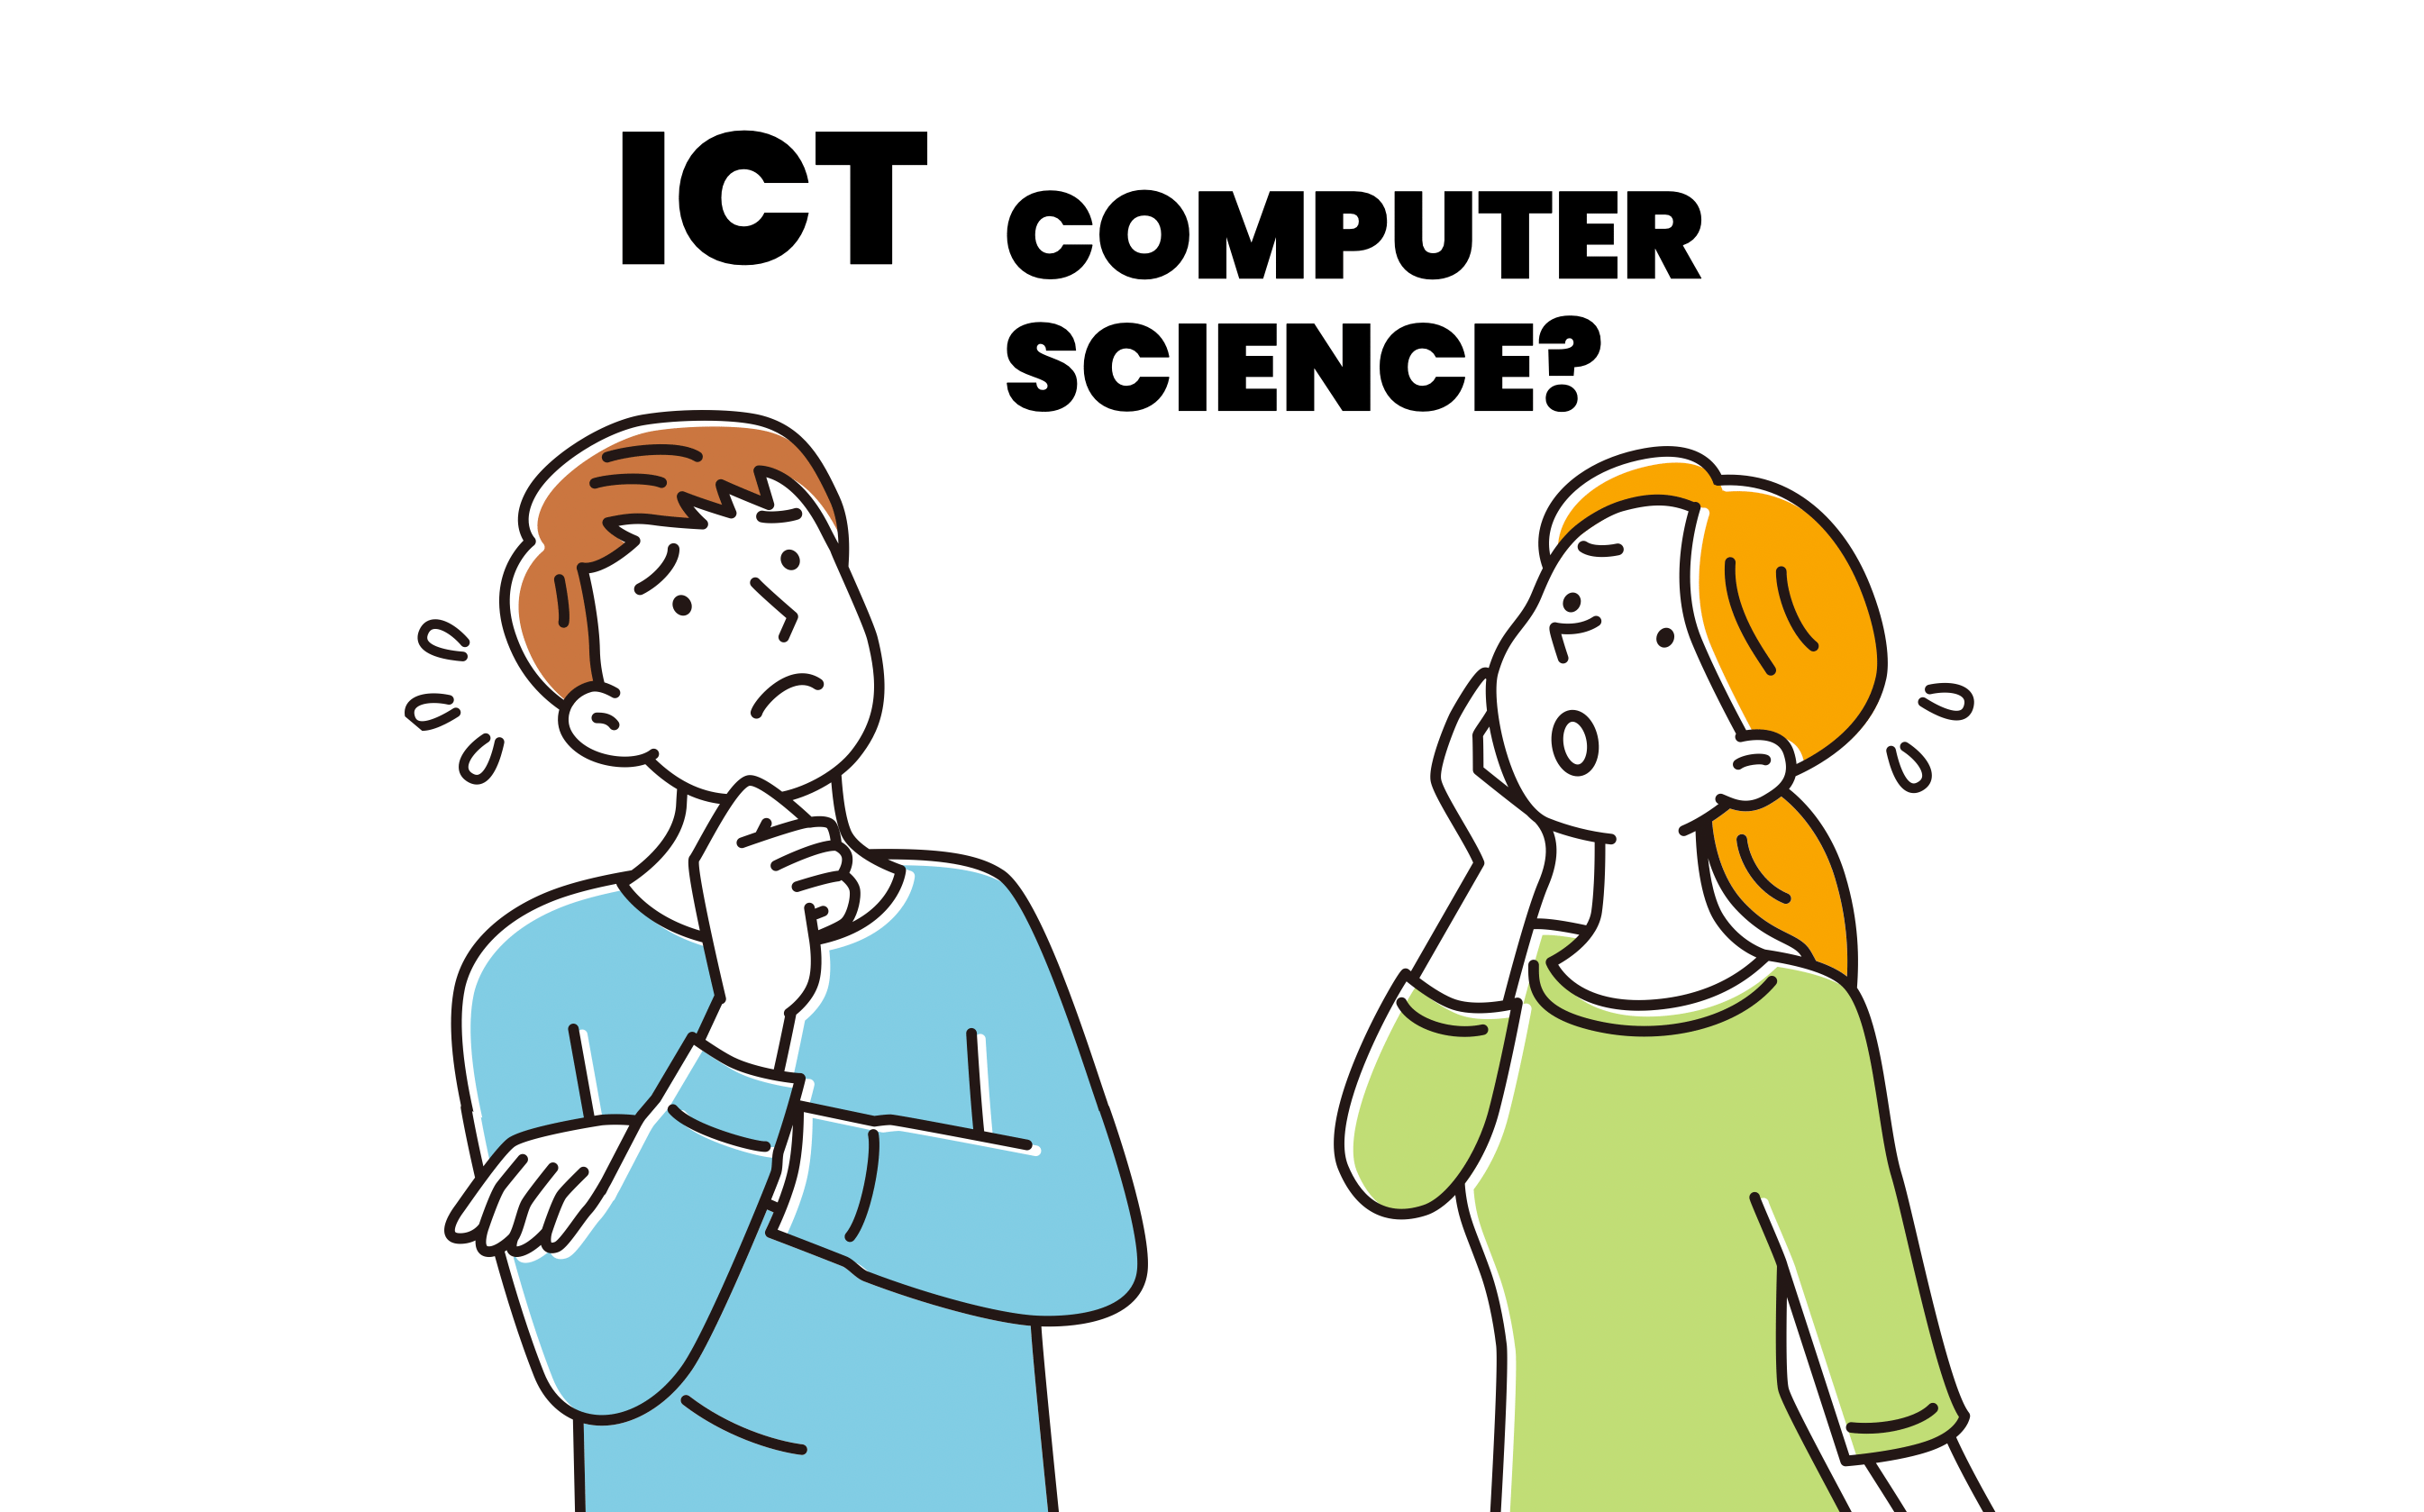
\includegraphics[scale=0.149]{Images/ictvscs.png}
\end{frame}


\begin{frame}
\begin{center}
\Huge Computer Science (CS)\\
\textbf { But what's the difference? }
\end{center}
\end{frame}


\begin{frame}{Lesson 1}{}
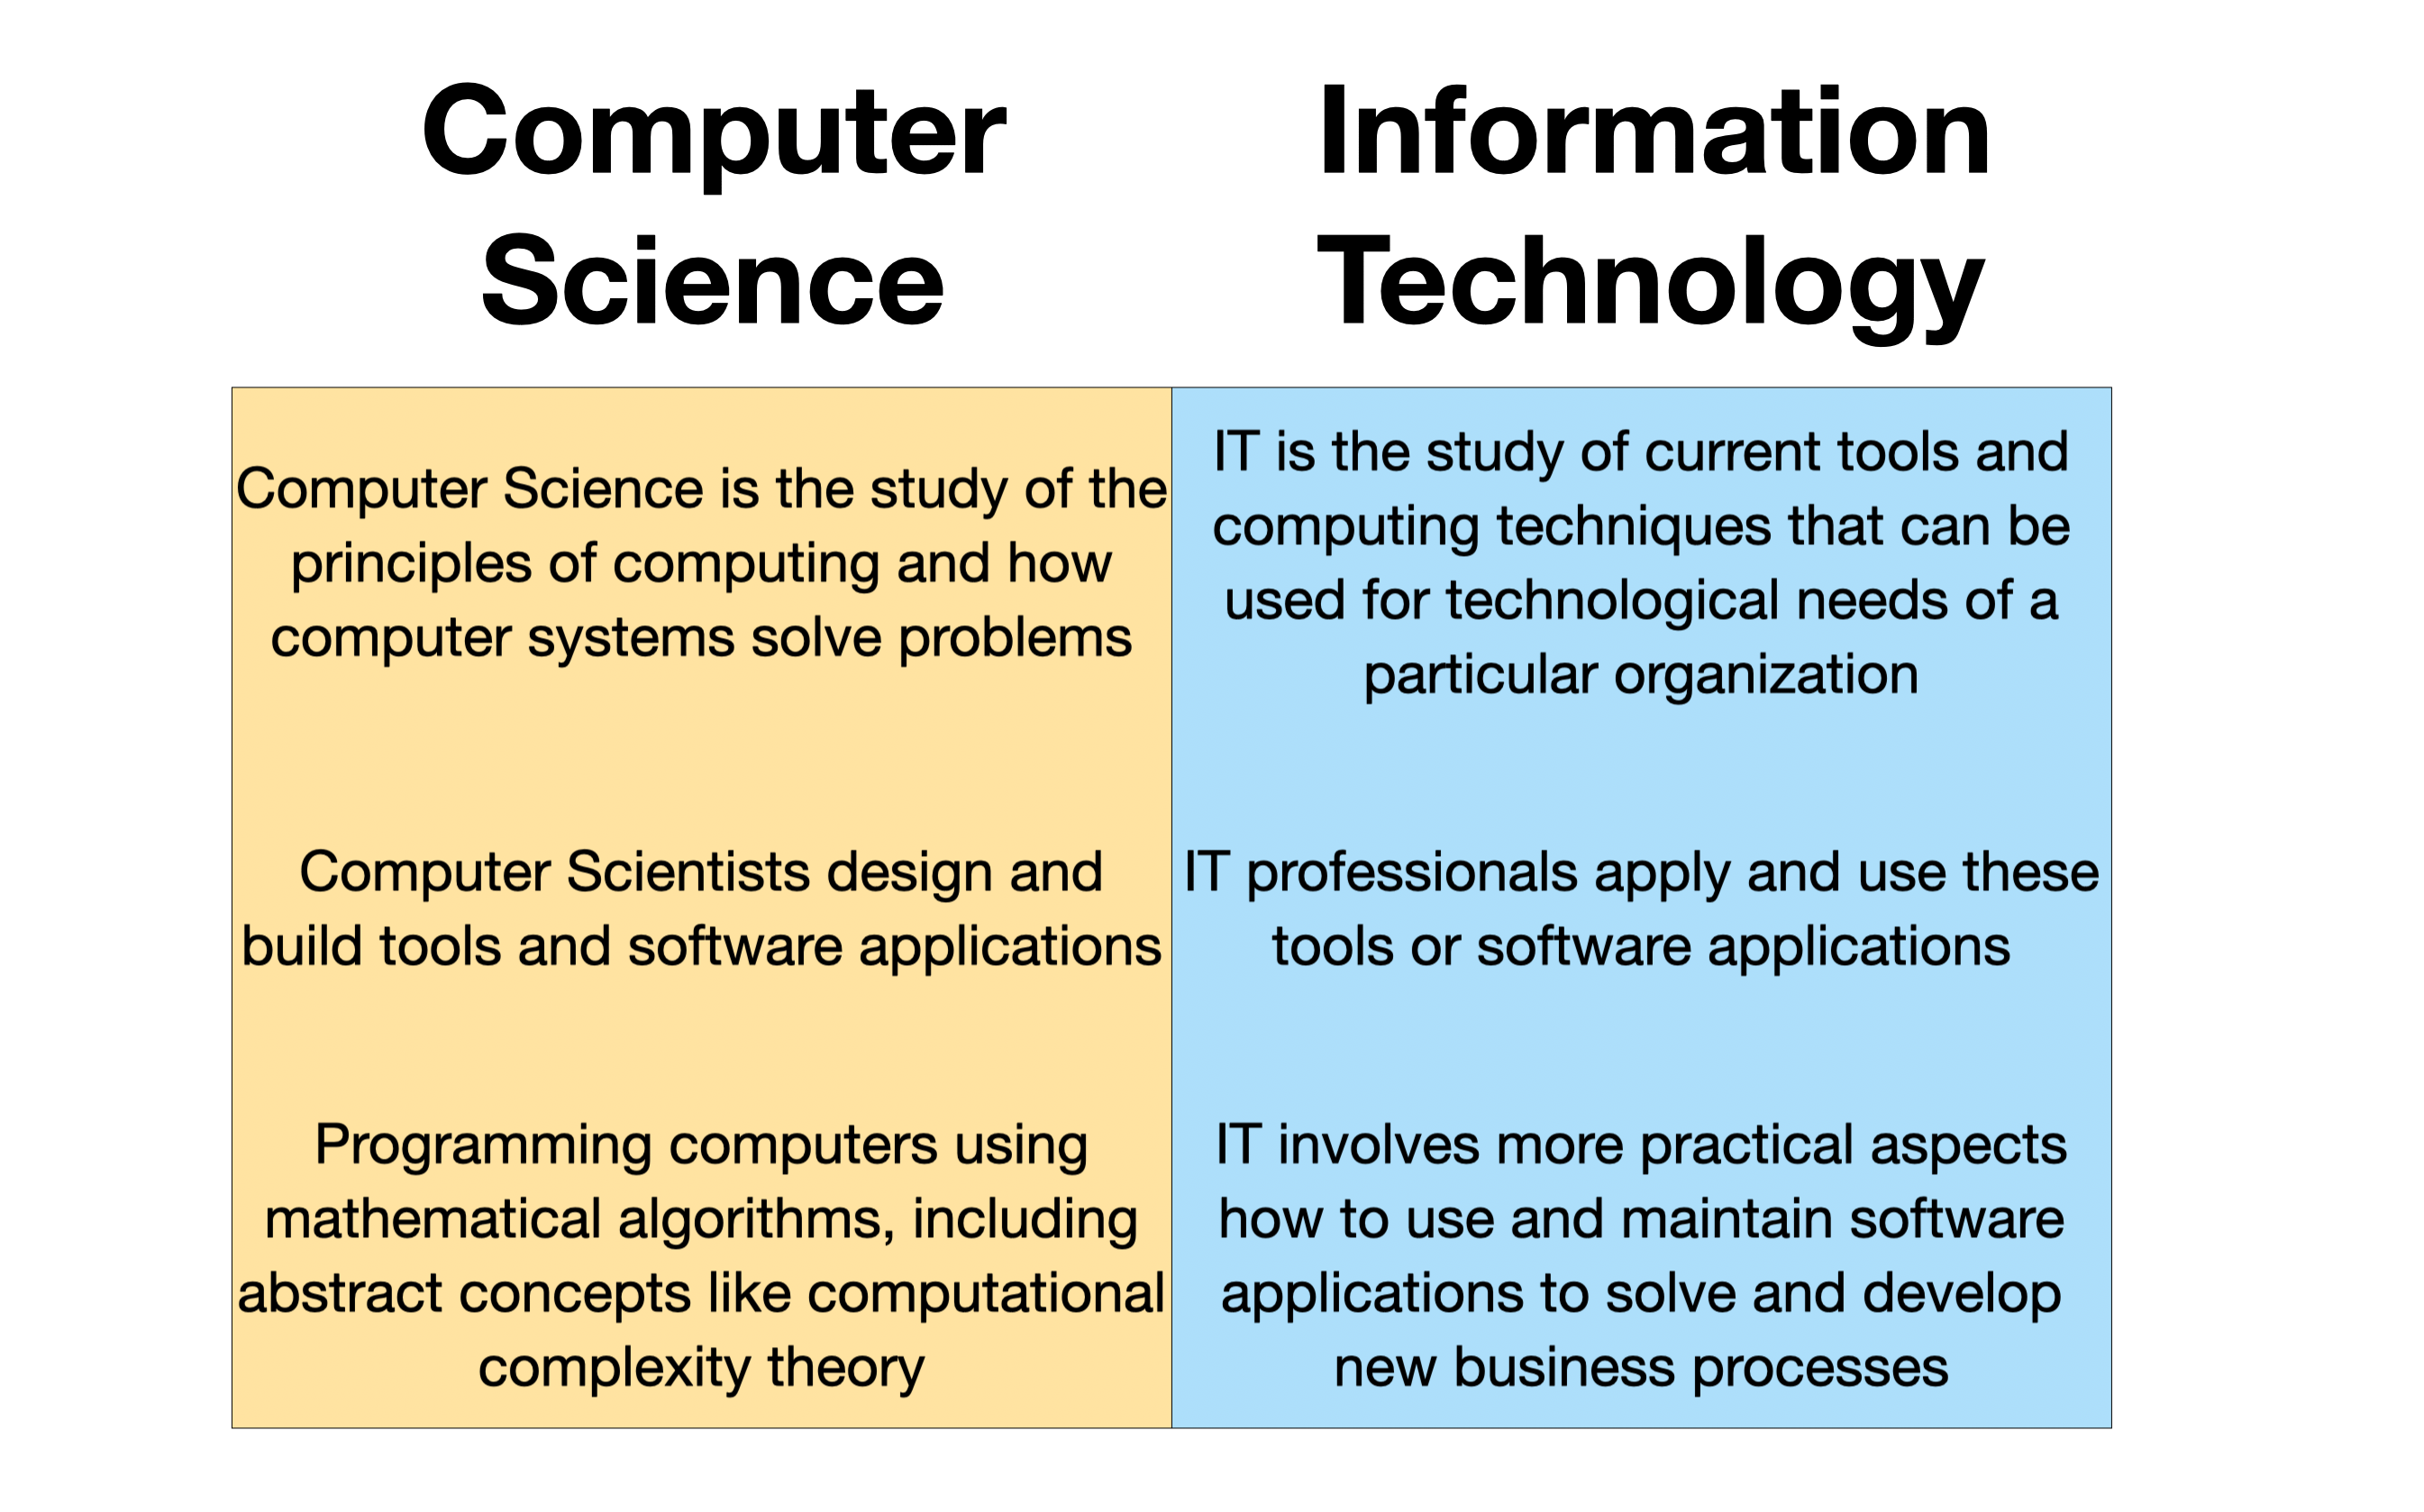
\includegraphics[scale=0.158]{Images/itvscs_10.png}
\end{frame}

\begin{frame}{Lesson 1}{}
\begin{center}
\Huge Computation
\end{center}
\end{frame}

\begin{frame}{Lesson 1}{}
{\Huge{What is a Computation?}}
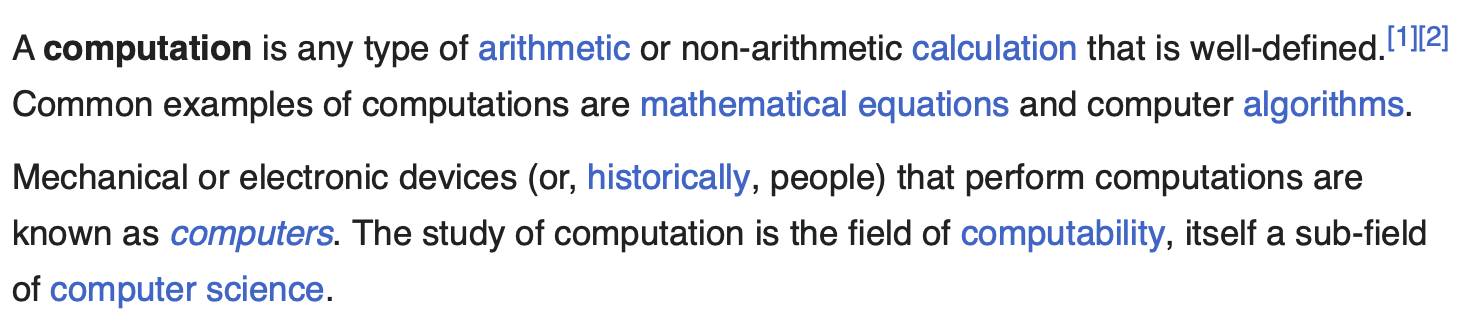
\includegraphics[scale=0.58]{Images/computation.png}
\end{frame}




\begin{frame}{Lesson 1}{}
\Large
A \textbf{computation} is what a computing device does, no matter of the computing device: a computer system, a tablet, a mobile phone.\\~\\

Example of computations: well-defined mathematical statements, which are solvable. But there are mathematically concepts which are not well-defined, and can be difficult to solve, like: the halting problem, or busy beaver game.

\end{frame}


\begin{frame}{Lesson 1}{}

\Large
Computing devices are supposed to compute something. Like calculate and predict the weather, render to produce a movie, browse the Internet.   \\~\\ 
Some well-defined computations:

\begin{itemize}
    \item calculations carried by an electronic computer or calculator
    \item calculations carried out on an \alert{analytical engine}
    \item majority of mathematical statements and calculations
\end{itemize}
\end{frame}


\begin{frame}{Lesson 1}{}
{\Large\textbf{{What is an Analytical Engine?}}}
\Large
\begin{minipage}{0.55\textwidth}
    \begin{itemize}
      \item The very first mechanical general-purpose computer
      \item Designed by the English mathematician and computer pioneer Charles Babbage
      \item Designed in 1837
    \end{itemize}
  \end{minipage}
\begin{minipage}{0.35\textwidth}
    % Show the image at item three and afterwards
      \begin{figure}
        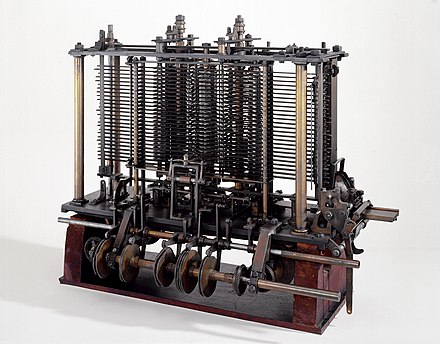
\includegraphics[scale=0.45]{Images/Babbages_AnalyticalEngine}
      \end{figure}
  \end{minipage}  
\end{frame}


\begin{frame}{Lesson 1}{}
{\Large\textbf{{The basic calculator}}}
\Large
\begin{minipage}{0.70\textwidth}
    \begin{itemize}
      \item Execute a number of precise operations
      \item Designed to contain a set of such operations and instructions
      \item Includes even more complex operations, graphing charting 
    \end{itemize}
  \end{minipage}
\begin{minipage}{.0\textwidth}
    % Show the image at item three and afterwards
      \begin{figure}
        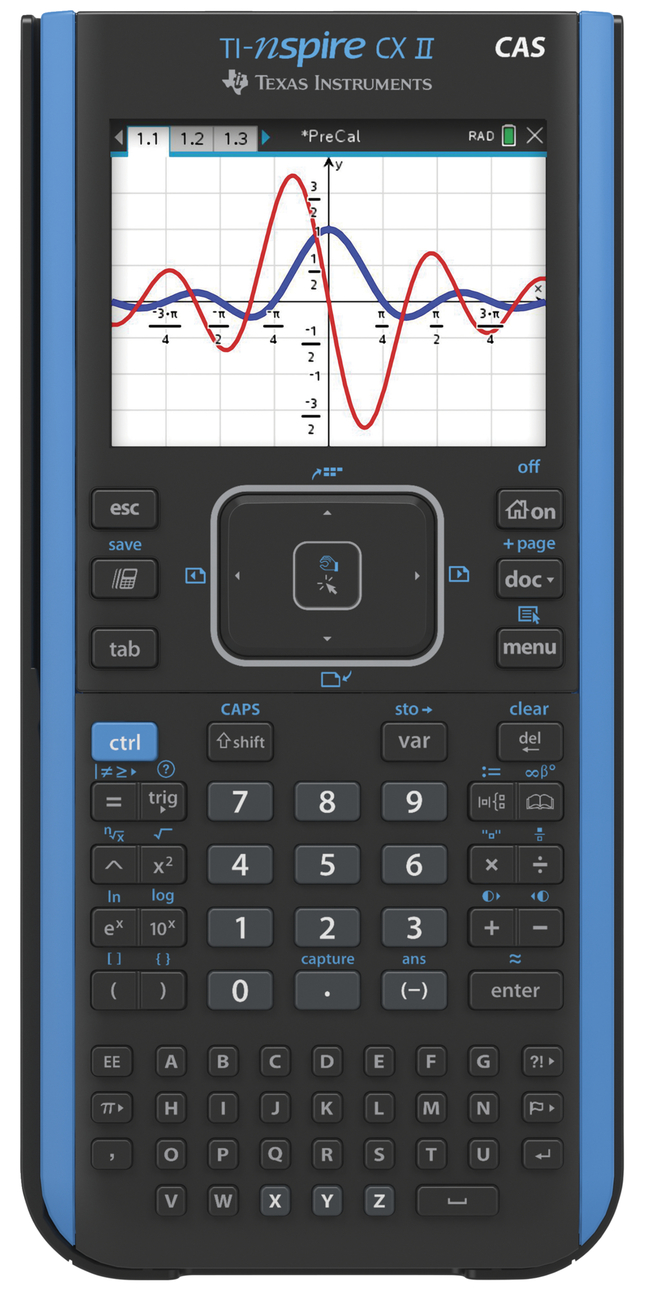
\includegraphics[scale=0.60]{Images/TI}
      \end{figure}
  \end{minipage}  
\end{frame}


\begin{frame}{Lesson 1}{}
\Large
\textbf{World's first computing device?}\\~\\ 
The escapement clock, a man-made device, to keep track of
time.\\~\\ 
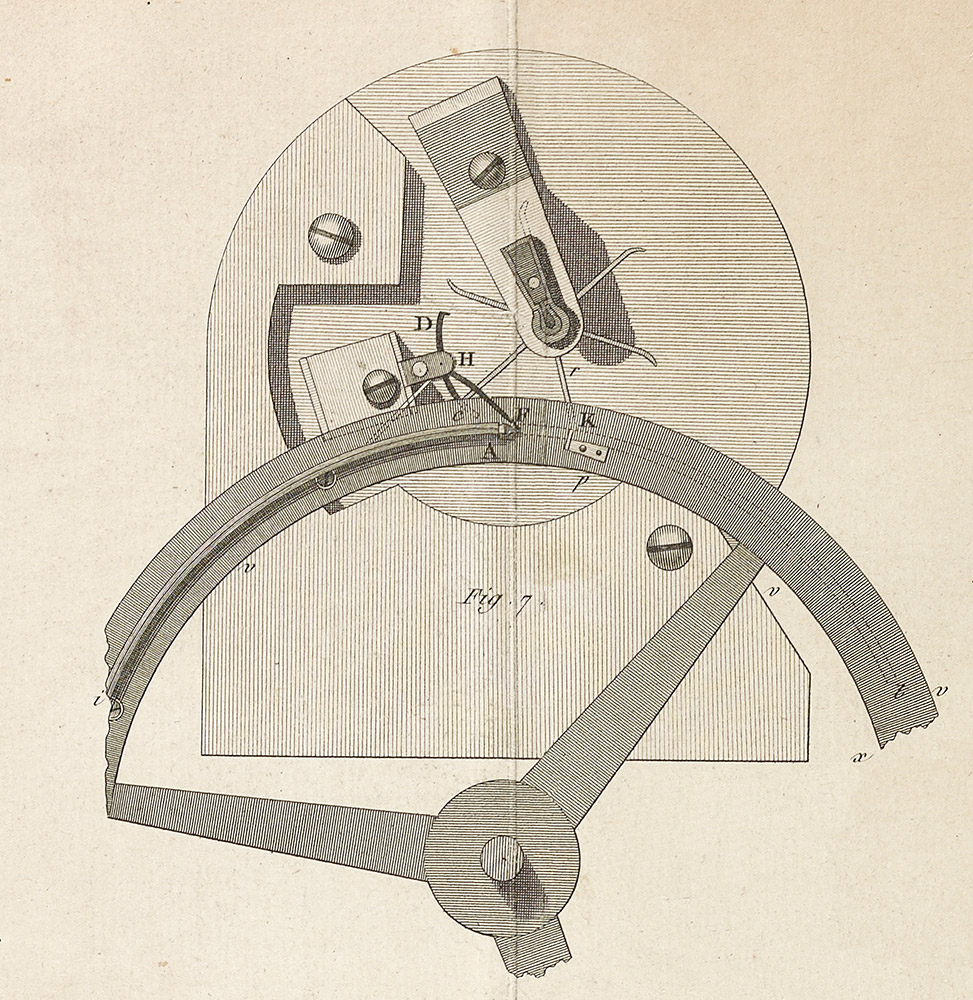
\includegraphics[scale=0.35]{Images/Le_Roy_escapement_mechanism}
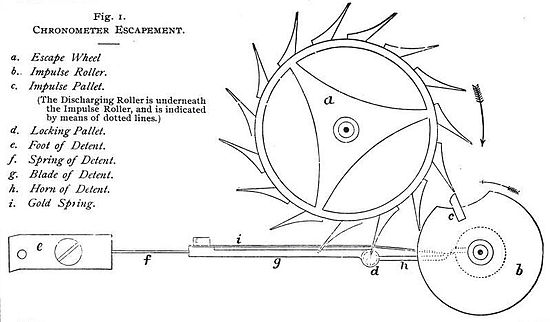
\includegraphics[scale=0.25]{Images/chronometer_detent_escapement}
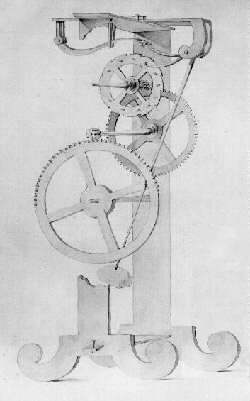
\includegraphics[scale=0.35]{Images/Galileo_Pendulum_Clock}
\end{frame}


\begin{frame}{Lesson 1}{}
\Large
Computation can be seen as a purely physical process occurring inside a closed \textbf{physical system} called a \textbf{computer}.\\~\\ 
Example of physical systems: analytical engine machines, human mathematicians following strict rules, digital computers, mechanical computers, analog computers and others.
\end{frame}


% --------------------------------------------------------------
% Algorithms 
% --------------------------------------------------------------
\begin{frame}{Lesson 1}{}
\begin{center}
\Huge Algorithms
\end{center}
\end{frame}

% What is an algorithm?
\begin{frame}{Lesson 1}{}
{\Huge{What is an algorithm?}}
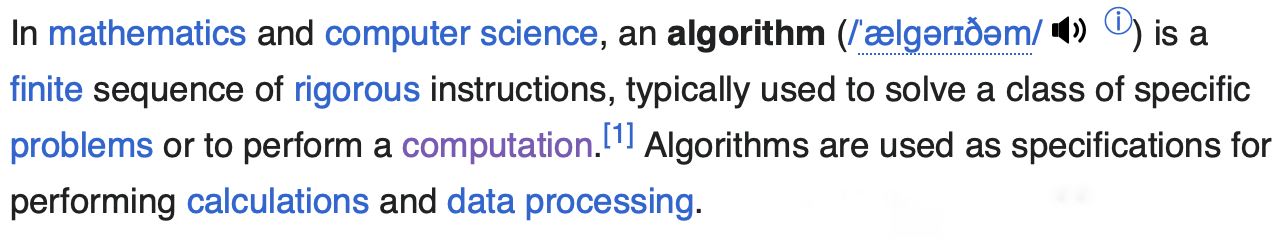
\includegraphics[scale=0.33]{Images/algorithm.png}

\Large{
\begin{itemize}
    \item But can we call this a \alert{computer program}?
    \item Or is it just a recipe, something higher than a \alert{sequence of code}
    \item A higher level of abstraction of how to implement something we plan to develop. Example: how to find a name in a phone book
\end{itemize}}

\end{frame}

\begin{frame}{Lesson 1}{Algorithms}
\Large
\textbf{Algorithms are everywhere}\\~\\ 
From your kitchen, in your microwave oven, your washing machine, to your phone or computer. When you browse Internet web sites your web browser is using different algorithms to decide how to display data to you.\\~\\
Our society relies on algorithms to suggest sentences for convicted criminals. You even use algorithms to keep you alive: the control systems from your car, or in different medical devices.
\end{frame}


\begin{frame}{Lesson 1}{Algorithms}
\Large
\textbf{But how can we describe them?}\\~\\ 
As an abstraction of something you plan to build or use, including all basic operations to achieve that. For example, think you plan to search in a phone book, a person phone number by the name:
\begin{itemize}
    \item you can start page by page searching for that name
    \item or you can jump directly to certain letters and start following from there
    \item or you can apply a different strategy, by 'cutting' the book into half, checking the letter in which half belongs, and applying all over again the same principle until the name is found
\end{itemize}
\end{frame}


\begin{frame}{Lesson 1}{Algorithms}
\Large
\textbf{How can we write one algorithm?}\\~\\ 
You can write it in plain English or in a more precise way using mathematics. Some others are using a form of \alert{pseudocode}.\\~\\
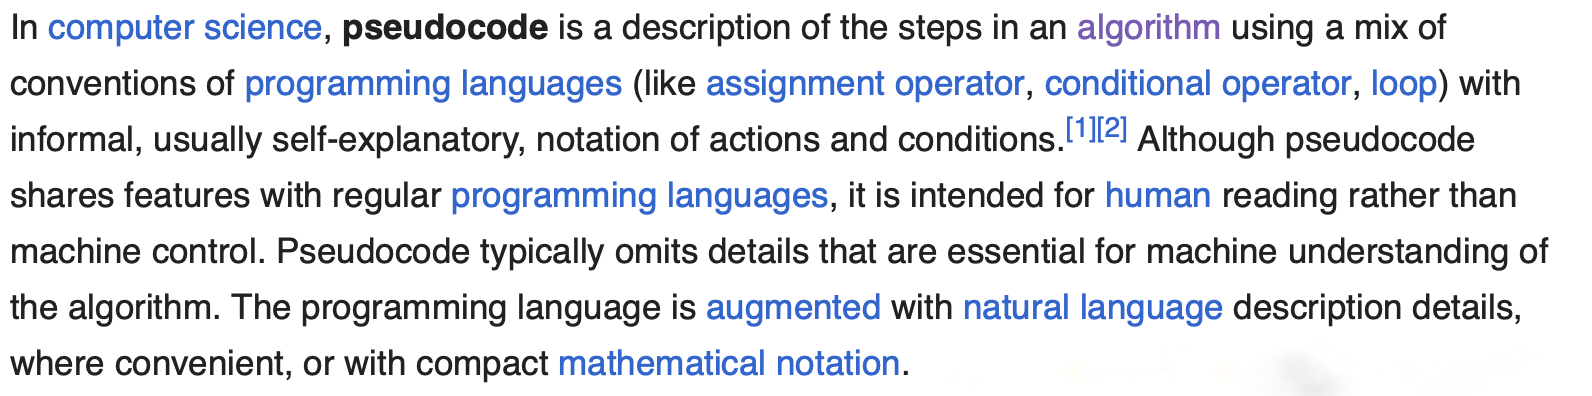
\includegraphics[scale=0.27]{Images/pseudocode}

\end{frame}


\begin{frame}{Lesson 1}{Algorithms}
\Large
\textbf{Example phonebook}\\~\\

\label{phonebook}

\begin{algorithmic}[1]

\Procedure{PhoneBook}{$N$}\Comment{Returns person name: N}
\State $N\gets 1$
\State Open page number $N$
\State Look at the page $N$
\If {Person is on page $N$}
    \State \textbf{Call person} $N$\Comment{The person name is $N$}
\Else \State \textbf{Find next page.} {$N\gets $N + 1} Go back to 3 
\EndIf
\EndProcedure
\end{algorithmic}
\end{frame}



\begin{frame}{Lesson 1}{Algorithms}
\Large
\textbf{But why not using a programming language?}\\~\\ 
We must think what we are planning to do, and how we plan to do it. And for that, we must not rely on a programming language: we will be restricted by the limits of the specific programming language not being able to design and think freely about it.\\~\\
A better approach is to think to write it as pseudocode or simple mathematics. This way we can have all flexibility and the power of precise mathematics.
\end{frame}



\begin{frame}{Lesson 1}{Algorithms}
\Large
\textbf{Euclid's Algorithm or GCD}\\~\\ 
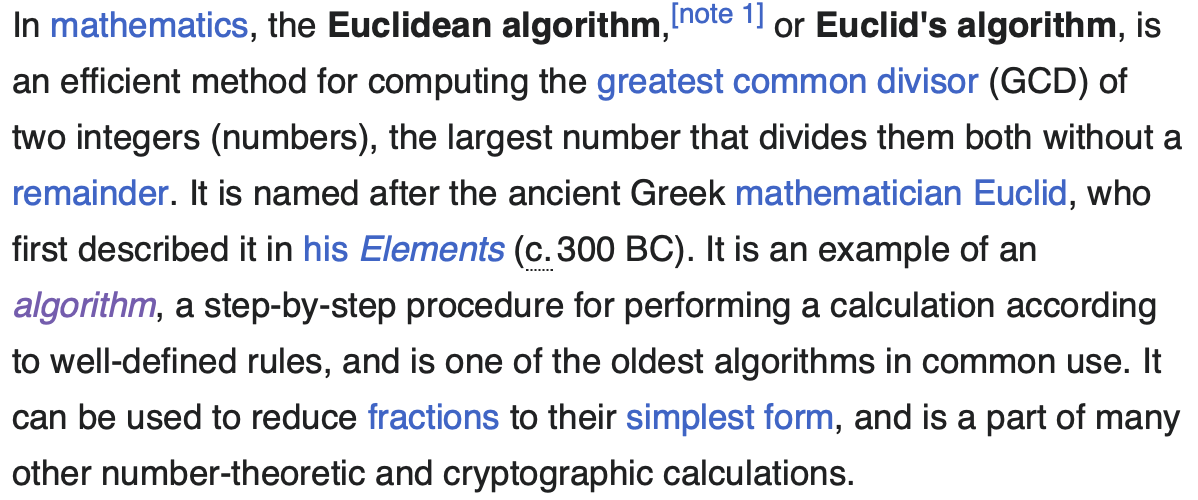
\includegraphics[scale=0.7]{Images/gcd}
\end{frame}

\begin{frame}{Lesson 1}{Algorithms}
\Large
\textbf{Euclid's Algorithm}\\~\\ 
Greatest Common Divisor (GCD) of two numbers A and B is the largest number that divides both A and B. (Number here defined as an \alert{integer})\\~\\

An integer is the number zero (0), a positive natural number (1, 2, 3, etc) or a negative integer with a minus sign (-1, -2, -3, etc) In mathematics we call this \(\mathbb{Z}\) set of numbers.
\end{frame}


\begin{frame}{Lesson 1}{Algorithms}
\Large
\textbf{Euclid's Algorithm}\\~\\
The very first version:\\~\\ 
If A = 0 then GCD(A,B)=B, since the GCD(0,B)=B, and STOP\\  
If B = 0 then GCD(A,B)=A, since the GCD(A,0)=A, and STOP\\  
Write A in quotient remainder form (A = B * Q + R)\\
Compute then GCD(B,R) since GCD(A,B) = GCD(B,R)
\end{frame}


\begin{frame}{Lesson 1}{Algorithms}
\Large
\textbf{Euclid's Algorithm, pseudocode}\\~\\

\label{GCD}
\begin{algorithmic}[1]
\Procedure{GCD}{$A,B$}\Comment{The g.c.d. of A and B}
   \State $R\gets A\bmod B$
   \While{$R\not=0$}\Comment{We have the answer if R is 0}
      \State $A\gets B$
      \State $B\gets r$
      \State $R\gets A\bmod B$
   \EndWhile\label{GCDendwhile}
   \State \textbf{return} $B$\Comment{The gcd is B}
\EndProcedure
\end{algorithmic}
\end{frame}



\begin{frame}{Lesson 1}{Algorithms}
\Large
\textbf{Euclid's Algorithm, improved}\\~\\

\label{Euclid}
\begin{algorithmic}[1]
\Procedure{Euclid}{$A,B$}\Comment{The g.c.d. of A and B}
\If{$B==0$}
    \State \textbf{return} $A$\Comment{The gcd is A}
\Else \State \textbf{return} \Call{Euclid}{$B, A\bmod B$}
\EndIf
\EndProcedure
\end{algorithmic}
\end{frame}



\begin{frame}{Lesson 1}{Algorithms}
\Large
\textbf{Euclid's Algorithm, using mathematics}\\~\\
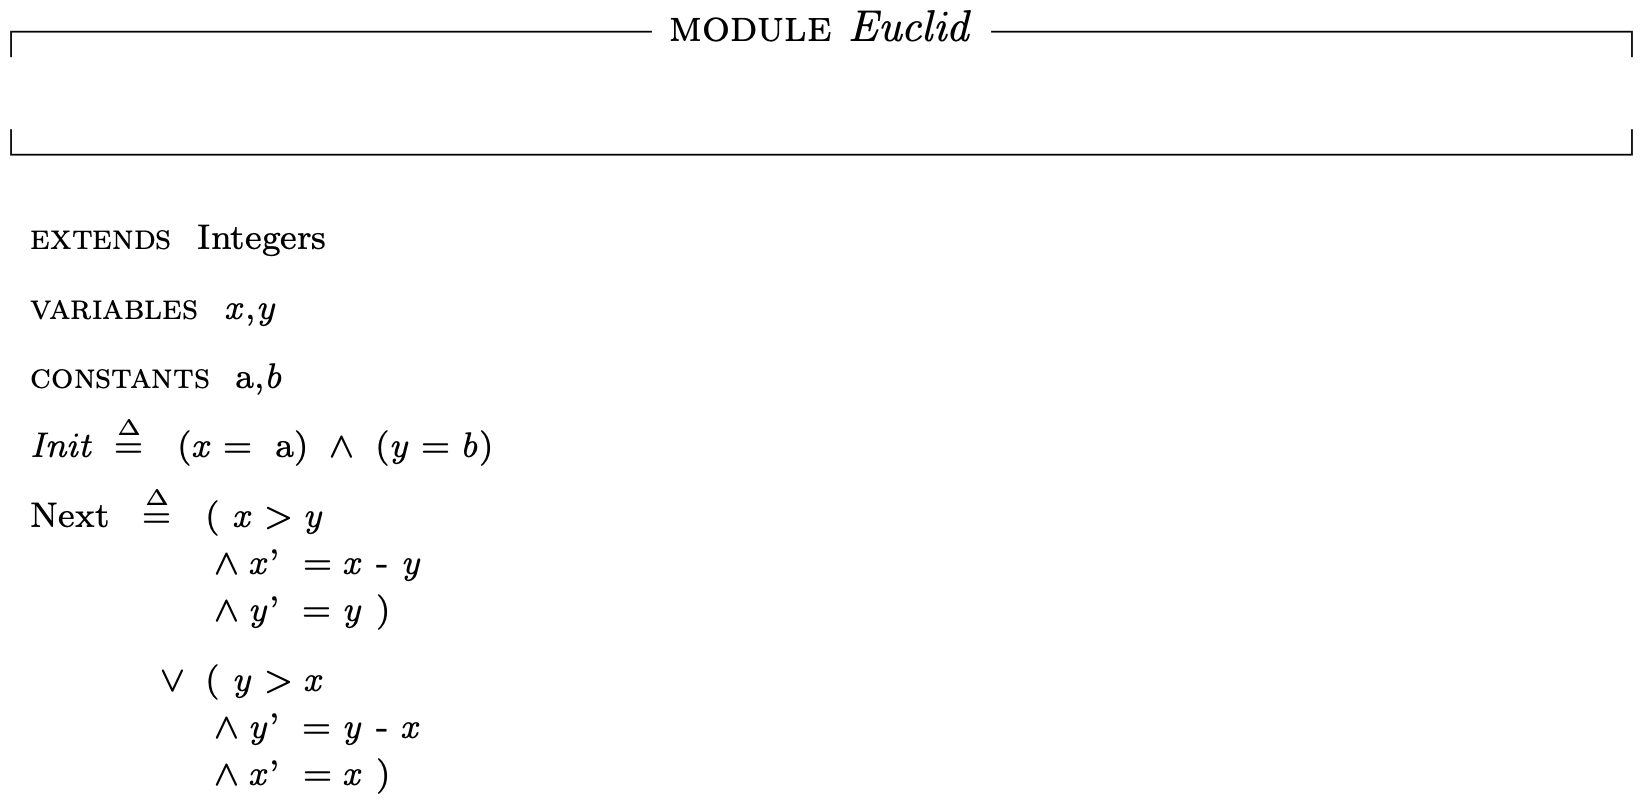
\includegraphics[scale=0.5]{Images/gcdtla}
\end{frame}


\begin{frame}{Lesson 1}{Algorithms}
\Large
\textbf{Classes of algorithms}\\~\\ 
    \begin{multicols}{3}
    \begin{itemize}
        \item Divide and Conquer
        \item Sorting
        \item Searching
        \item Dynamic programming
        \item Greedy algorithms
        \item Graph algorithms
        \item Shortest path
        \item Maximum flow
        \item Parallel algorithms
        \item Matrix operations
        \item Online algorithms
        \item Machine learning
        \item Linear programming
        \item String matching
    \end{itemize}
    \end{multicols}
\end{frame}



% --------------------------------------------------------------
% Programs 
% --------------------------------------------------------------
\begin{frame}{Lesson 1}{}
\begin{center}
\Huge Computer Programs
\end{center}
\end{frame}


% What is a computer program?
% What is an algorithm?
\begin{frame}{Lesson 1}{}
{\Huge{What is a computer program?}}
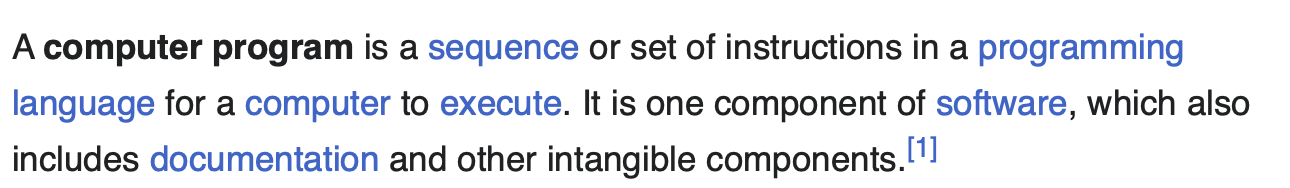
\includegraphics[scale=0.67]{Images/program}

\Large{
\begin{itemize}
    \item A computer program in its human-readable form: source code
    \item The source code needs to be translated into machine code to be able to execute
    \item The resulting file is called an executable file
    \item Then the operating system loads the executable into memory and starts a process to execute it
\end{itemize}}

\end{frame}


\begin{frame}{Lesson 1}{Algorithms}
\Huge Computers, digital systems are executing programs
\end{frame}


\begin{frame}{Lesson 1}{Programs}
\Large
\textbf{From source code to executable}\\~\\ 
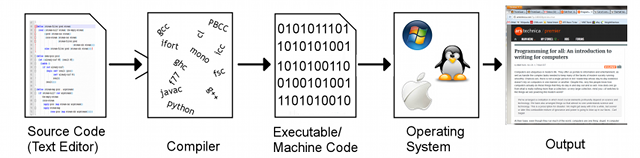
\includegraphics[scale=0.65]{Images/CompilationChain}
\end{frame}


\begin{frame}{Lesson 1}{}
{\Huge{Program structure}}
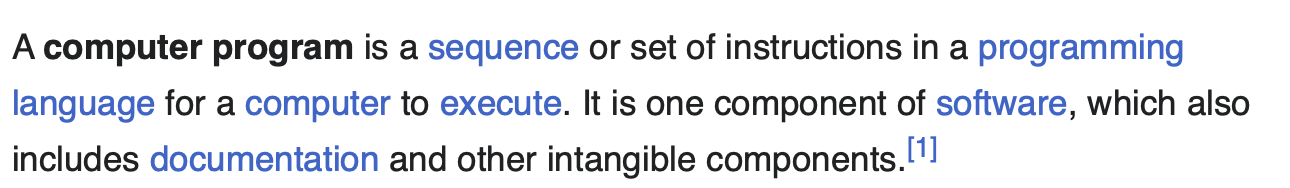
\includegraphics[scale=0.67]{Images/program}

\Large{
\begin{itemize}
    \item Some programs run forever, some dont
    \item A program execution is defined by at least one computation
    \item A computation is a sequence of states
    \item And a state is an assignment of values to variables
\end{itemize}}

\end{frame}


\begin{frame}{Lesson 1}{}
{\Huge{Program types}}\\~\\ 

\Large{
\begin{itemize}
    \item A program is modelled by a set of computations, representing all possible executions
    \item Remember an algorithm is just an abstract program
    \item Different programs: software applications and system software
    \item System software: operating systems
\end{itemize}}
\end{frame}


\begin{frame}{Lesson 1}{}
{\Large\textbf{{Application and System Programs}}}

\Large
\begin{minipage}{0.65\textwidth}
    \begin{itemize}
      \item \textbf{Software applications}:  enterprise resource planning, customer relationship management, supply chain management software, web, middleware, databases
      \item \textbf{Operating systems}: macOS, RedHat, FreeBSD, Windows
    \end{itemize}
  \end{minipage}
\begin{minipage}{0.30\textwidth}
    % Show the image at item three and afterwards
      \begin{figure}
        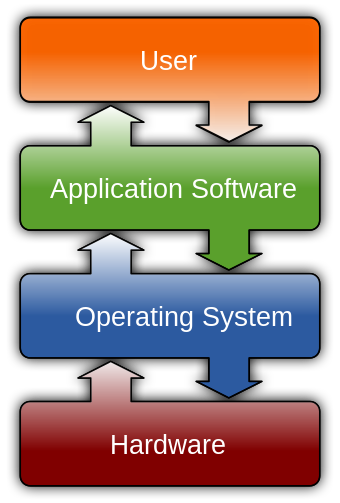
\includegraphics[scale=0.32]{Images/OS}
      \end{figure}
  \end{minipage}
\end{frame}


\begin{frame}{Lesson 1}{Programs}
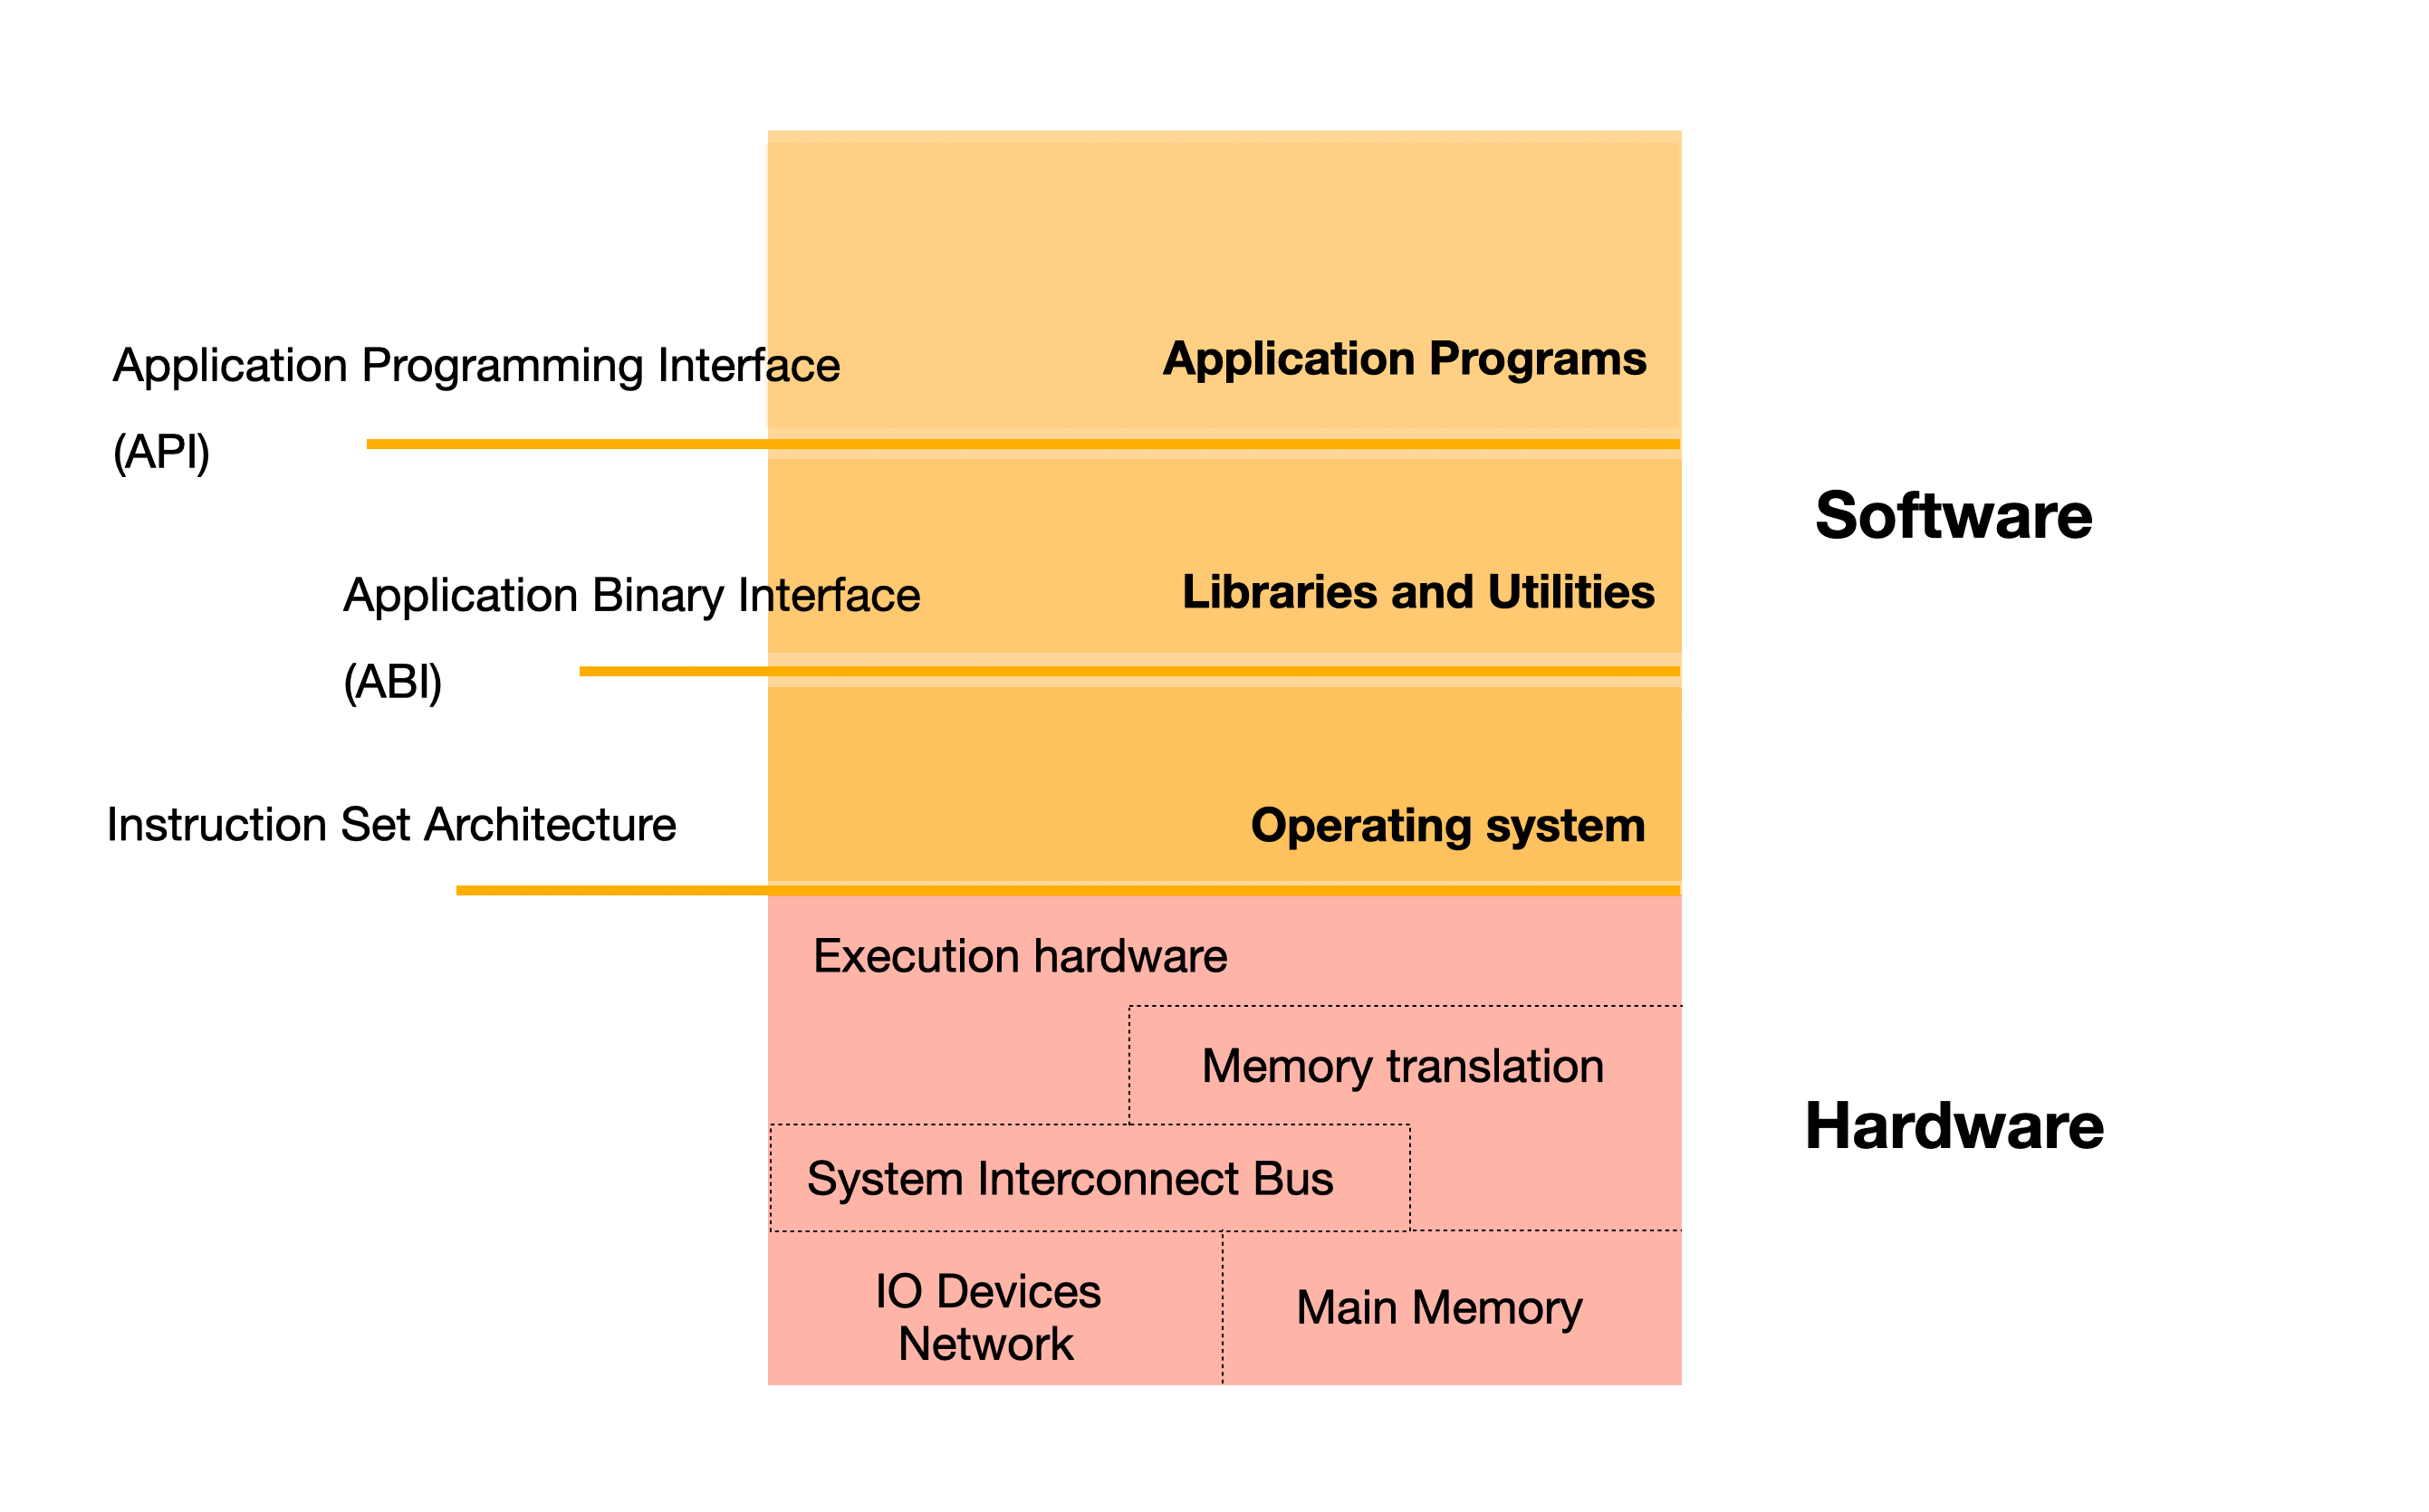
\includegraphics[scale=0.15]{Images/sfwhdw}
\end{frame}


\end{document}

